\documentclass[12pt]{article}

\usepackage{amsmath}
\usepackage{amssymb}
% \usepackage{fullpage}
\usepackage{graphicx}

\addtolength{\oddsidemargin}{-.875in}
\addtolength{\evensidemargin}{-.875in}
\addtolength{\textwidth}{1.75in}
\addtolength{\topmargin}{-1in}
\addtolength{\textheight}{2in}

\begin{document}

\section*{Galaxy-galaxy lensing by galaxies in clusters}

The galaxy-galaxy lensing signal is measured by azimuthally averaging the shapes of background sources around foreground, lens galaxies. This azimuthal averaging ensures that, at scales small enough where the cluster potential is approximately constant, the contribution to the lensing signal from the cluster itself is exactly zero. At larger distances from the galaxy, approaching the distance to the cluster centre, the cluster contribution rapidly takes over and dominates the signal. However, we do not expect any contribution from the galaxy itself at these scales, so effectively the two contributions are independent; this is shown in Fig.\ 1 (see also Fig.\ 6 of Sif\'on et al.\ 2015 for a demonstration that tbe two mass estimates are uncorrelated).

Therefore, to measure the lensing signal arising from galaxies in clusters one must have a high source density because the signal from the galaxy is noticeable only at very small scales ($\lesssim100$ kpc, depending on the distance from the galaxy to the cluster centre). We are able to do this thanks to our deep, low-seeing ($\lesssim0.8''$) CFHT images. Fig.\ 3 shows the stellar-to-total mass relation for all galaxies in the MENeaCS cluster sample, from which our UDG sample is drawn. This has been obtained from measurements around 8,000 spectroscopically-confirmed cluster galaxies (Sif\'on et al., 2016a, in prep.). Fig.\ 4 shows our preliminary measurement of the lensing signal of UDGs in a subsample of the clusters entering Fig.\ 3 (Sif\'on et al.\ 2016b, in prep.), with the best-fit model overlaid. The systematic uncertainties in the lensing \emph{measurements} (including shape measurement and photometric redshift uncertainties) have been quantified by Hoekstra et al.\ (2015) to be about 7\%. The major systematic is therefore in our \emph{interpretation} of the measurement, as we do not know what fraction of these galaxies is really in the cluster: there is \emph{no spectroscopy availablbe for UDGs}, except for the one example mentioned in the proposal. This is the main goal of our proposed observations: to understand what fraction of the selected UDGs are really part of the cluster. A significant fraction of background galaxies in our sample would imply a high contamination of our lensing measurements, as background galaxies would be more massive than we infer by assuming they are at the cluster redshift.




\pagebreak

\begin{figure}
 \centerline{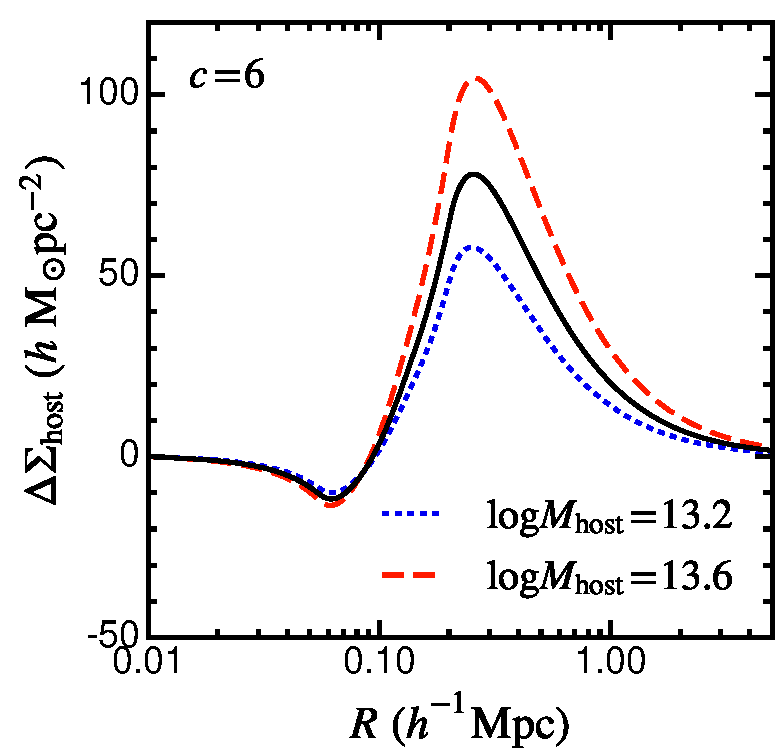
\includegraphics[width=2.5in]{ESDhost_bin1_cfix.pdf}
             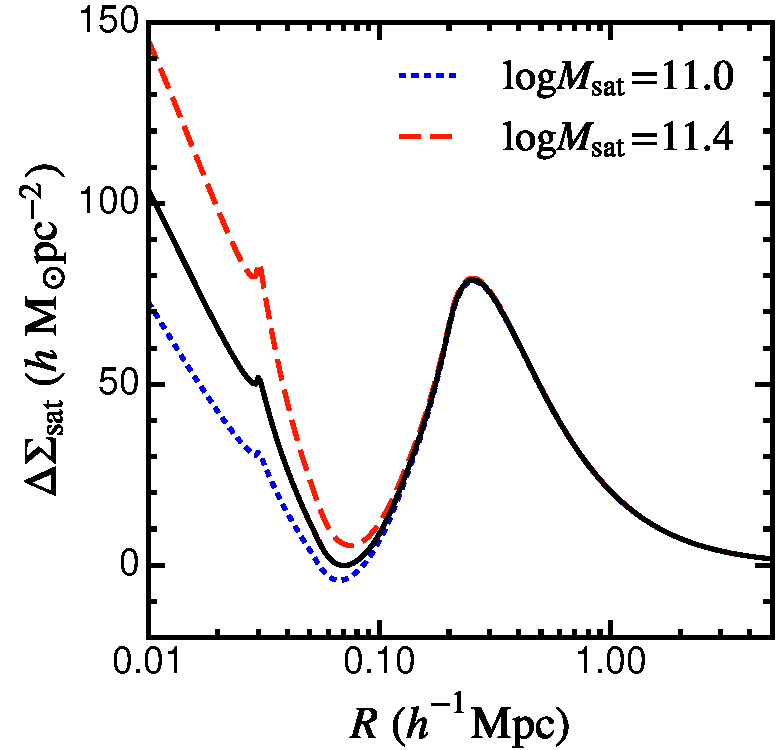
\includegraphics[width=2.5in]{ESDsat_bin1_msat.pdf}}
\caption{\small Left: predicted lensing signal of clusters with masses $\log M_{\rm host}/M_\odot=13.2,13.4,13.6$. Changing the cluster mass only changes the amplitude of the signal but not the scale at which it is different from zero. Right: predicted signal of galaxies of mass $\log M_{\rm sat}/M_\odot=11.0,11.2,11.4$ in a cluster with $\log M_{\rm host}/M_\odot=13.4$ at a distance $R_{\rm sat}\sim100\,{\rm kpc}$ from the cluster centre. The glitch is produced by the sharp truncation assumed for the galaxy. Taken from Sif\'on et al.\ (2015, MNRAS, 454, 3938).}
\end{figure}

\begin{figure}
 \centerline{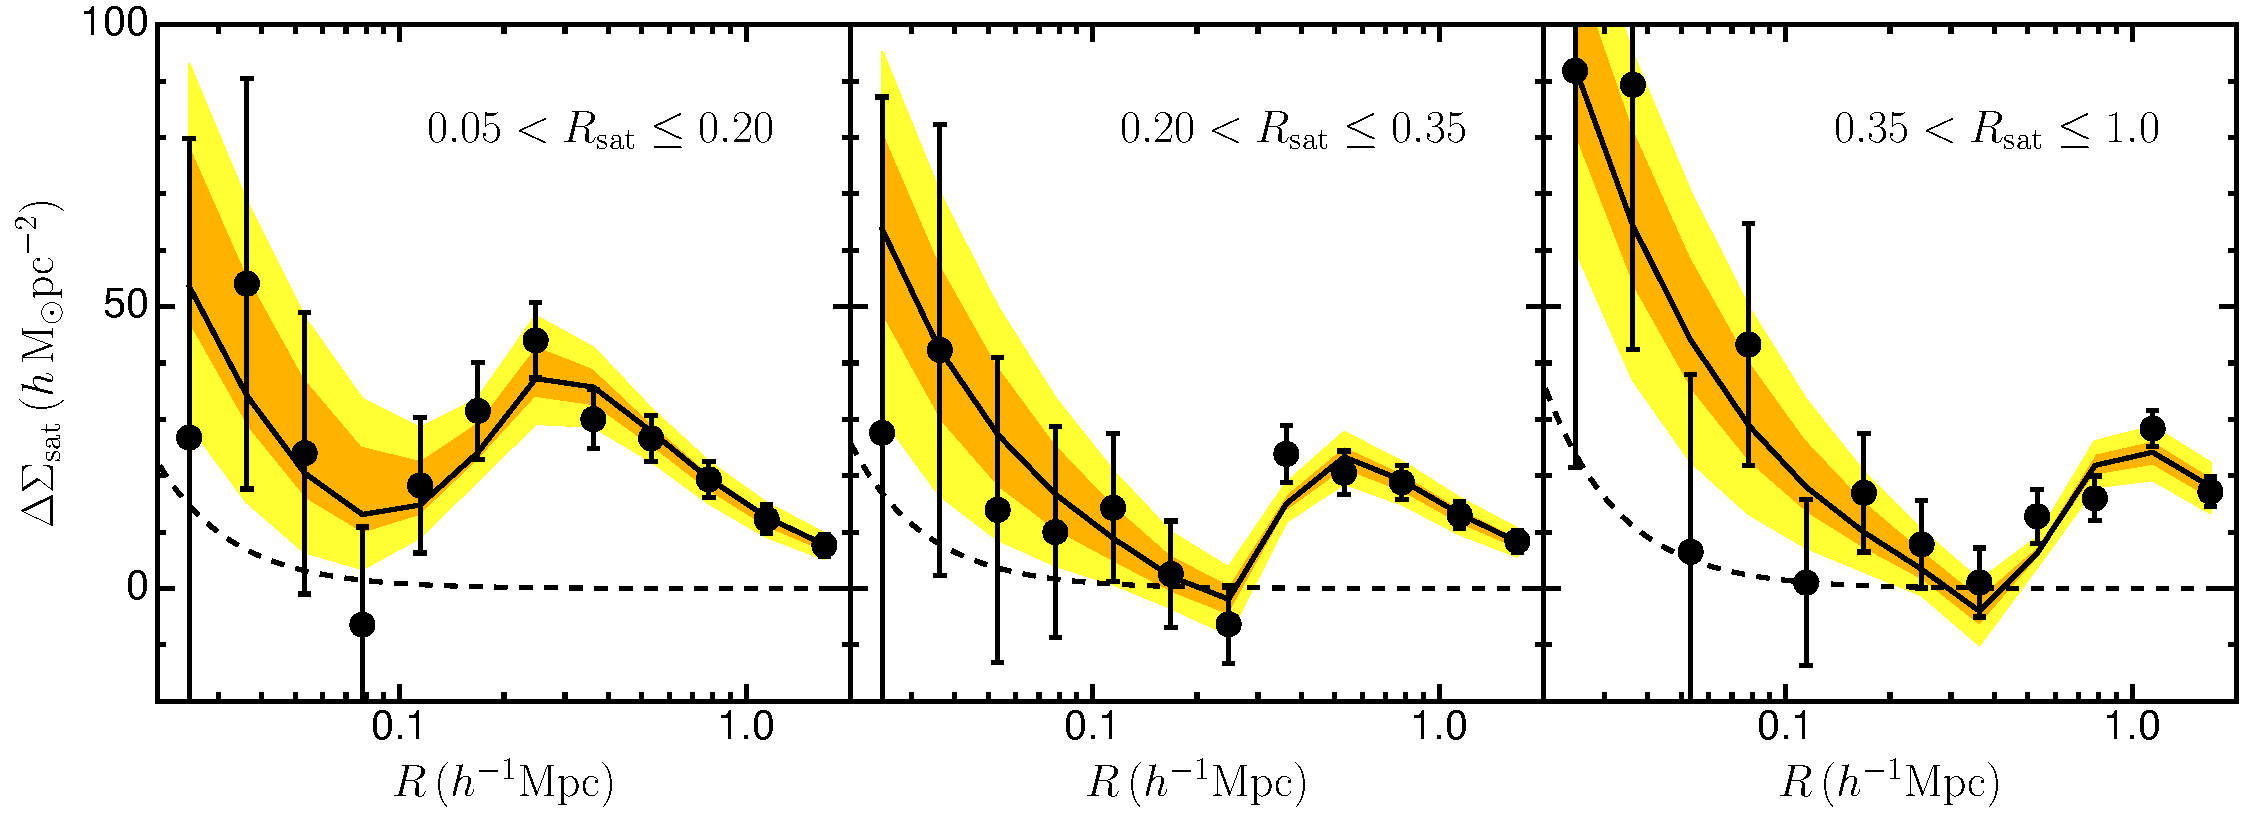
\includegraphics[width=6in]{esd_kids.pdf}}
\caption{\small Lensing signal of galaxies in low-mass galaxy clusters identified in the GAMA survey, using background sources from the Kilo-Degree Survey. Contours show 68 and 95\% credible intervals of best-fit NFW profiles obtained through an MCMC. The best-fit masses of galaxies in the three panels (separated by distance to the cluster centre as shown in the legend) are $\log M_{\rm sat}/M_\odot=11.8,11.8,12.2$. The dashed lines show the signal predicted by the average stellar masses of galaxies in each bin (the cluster contribution is not included). Note how the signal from the cluster moves to larger scales for galaxies further away from the centre.}
\end{figure}

\begin{figure}
 \centerline{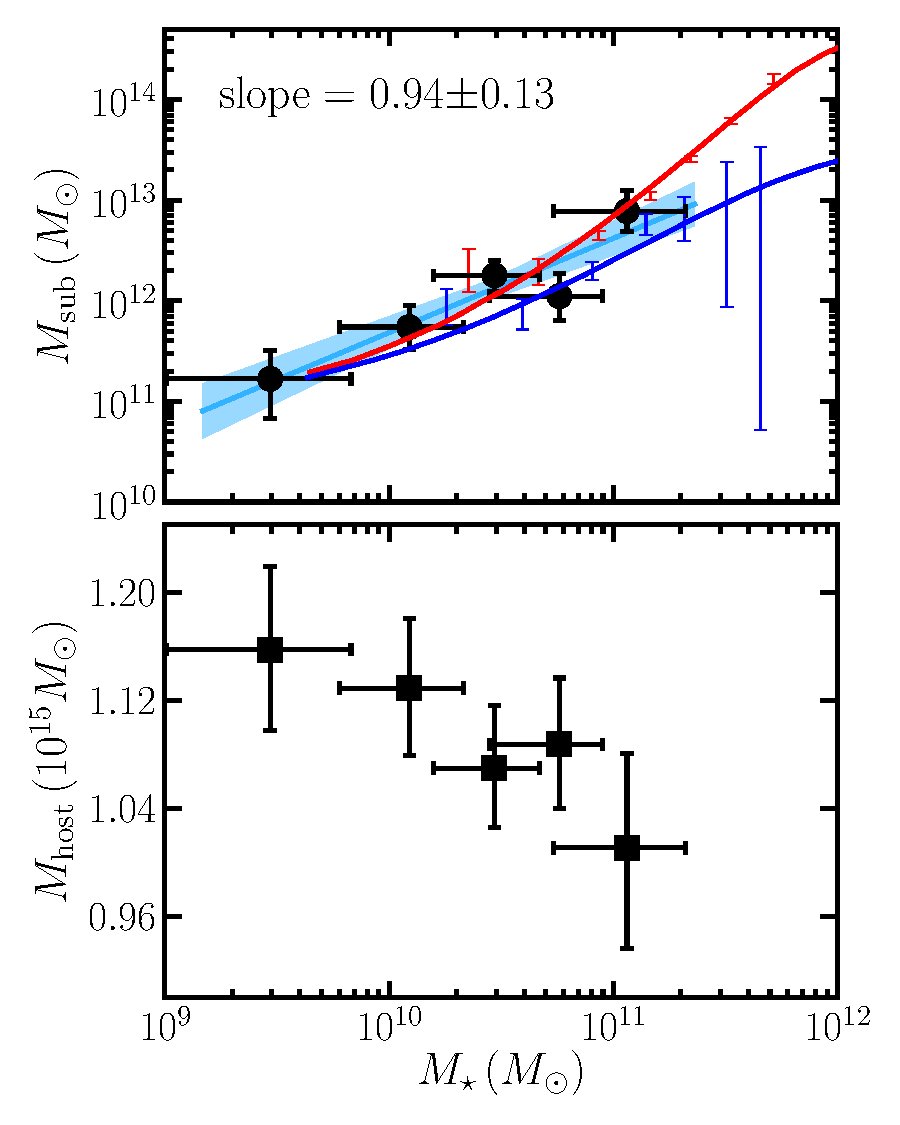
\includegraphics[width=3in]{mass_mstar.pdf}
             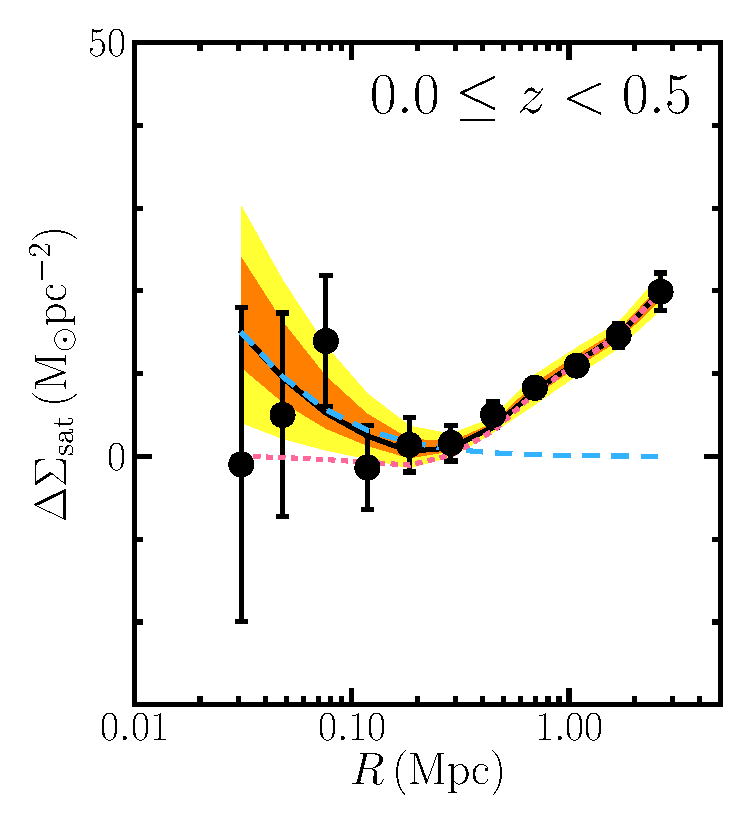
\includegraphics[width=3in]{esd.pdf}}
\caption{\small Left: stellar-to-total mass relation of the general population of cluster galaxies in massive clusters (blue band), obtained by fitting the lensing signal of satellites in each stellar mass bin (black points). Blue and red errorbars show measurements of the same relation for blue and red \emph{central} galaxies in SDSS, and the blue and red lines show predictions from numerical simulations. {\bf you can cut out the lower panel which shows cluster masses.} Right: lensing measurement of UDGs identified by vdB+16. The signals arising from the galaxy (blue dashed) and from the cluster (red dotted) can be clearly distinguished.}
\end{figure}


\end{document}
